\documentclass[tikz,border=2mm]{standalone}
\usepackage{amssymb}
\usetikzlibrary{arrows.meta,calc,decorations.pathmorphing}

\definecolor{ink}{HTML}{183B50}
\definecolor{water}{HTML}{EAF3F4}
\definecolor{teal}{HTML}{087D79}
\definecolor{orange}{HTML}{C46B35}
\definecolor{warm}{HTML}{FFF4EA}
\definecolor{muted}{HTML}{60707A}
\definecolor{blue}{HTML}{3C7CA2}

\tikzset{
  panel/.style={draw=ink!22,rounded corners=5pt,fill=white,line width=.7pt},
  tinyarrow/.style={-{Stealth[length=2.2mm]},line width=1.05pt},
  flowarrow/.style={-{Stealth[length=3mm]},line width=1.45pt},
  microdot/.style={circle,inner sep=0pt,minimum size=2.5pt,fill=ink},
}

% An original qualitative diagram: the panels are three descriptions of the
% same class of models, not successive states of one trajectory.
\begin{document}
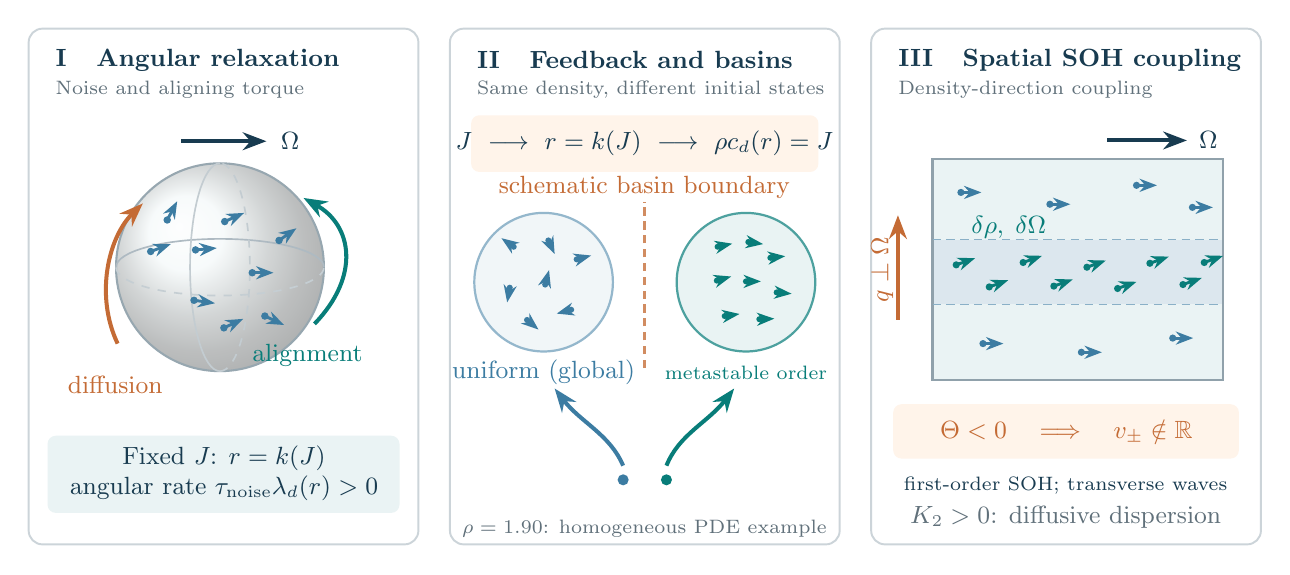
\begin{tikzpicture}[x=1cm,y=1cm]
  \draw[panel] (0,0) rectangle (4.95,6.55);
  \draw[panel] (5.35,0) rectangle (10.30,6.55);
  \draw[panel] (10.70,0) rectangle (15.65,6.55);

  % I. Frozen-field angular dynamics on a sphere.
  \node[anchor=west,font=\bfseries\small,text=ink] at (.22,6.15)
    {I\quad Angular relaxation};
  \node[anchor=west,font=\scriptsize,text=muted] at (.22,5.77)
    {Noise and aligning torque};
  \shade[ball color=water,opacity=.48] (2.43,3.52) circle (1.32);
  \draw[ink!45,line width=.75pt] (2.43,3.52) circle (1.32);
  \draw[ink!25,dashed,line width=.6pt] (1.11,3.52) arc[start angle=180,end angle=360,x radius=1.32,y radius=.36];
  \draw[ink!35,line width=.6pt] (1.11,3.52) arc[start angle=180,end angle=0,x radius=1.32,y radius=.36];
  \draw[ink!26,line width=.6pt] (2.43,4.84) arc[start angle=90,end angle=270,x radius=.38,y radius=1.32];
  \draw[ink!26,dashed,line width=.6pt] (2.43,2.20) arc[start angle=-90,end angle=90,x radius=.38,y radius=1.32];
  % Direction-bearing particles: vectors remain distributed on S^d.
  \foreach \x/\y/\angle in {
    1.55/3.72/20,1.76/4.12/62,2.10/3.10/-8,
    2.49/4.10/24,2.84/3.45/0,3.18/3.86/35,
    3.00/2.90/-25,2.12/3.74/5,2.48/2.75/25}
  {\fill[blue] (\x,\y) circle (1.35pt);
   \draw[tinyarrow,blue] (\x,\y) -- ++(\angle:.27);}
  \draw[flowarrow,orange] (1.13,2.55) .. controls (.84,3.16) and (1.01,3.90) .. (1.45,4.33);
  \node[font=\small,text=orange] at (1.10,2.02) {diffusion};
  \draw[flowarrow,teal] (3.63,2.80) .. controls (4.21,3.40) and (4.12,4.05) .. (3.49,4.40);
  \node[font=\small,text=teal] at (3.54,2.40) {alignment};
  \draw[flowarrow,ink] (1.94,5.12) -- (3.02,5.12);
  \node[anchor=west,font=\small,text=ink] at (3.08,5.12) {$\Omega$};
  \fill[water,rounded corners=3pt] (.24,.40) rectangle (4.71,1.38);
  \node[align=center,font=\small,text=ink] at (2.48,.90)
    {Fixed $J$: $r=k(J)$\\
     angular rate $\tau_{\rm noise}\lambda_d(r)>0$};

  % II. Self-consistent feedback and two basins at the same density.
  \begin{scope}[shift={(5.35,0)}]
    \node[anchor=west,font=\bfseries\small,text=ink] at (.22,6.15)
      {II\quad Feedback and basins};
    \node[anchor=west,font=\scriptsize,text=muted] at (.22,5.77)
      {Same density, different initial states};
    \fill[warm,rounded corners=3pt] (.27,4.73) rectangle (4.68,5.45);
    \node[font=\small,text=ink] at (2.47,5.09)
      {$J\ \longrightarrow\ r=k(J)\ \longrightarrow\ \rho c_d(r)=J$};
    \draw[orange!78,densely dashed,line width=.95pt] (2.47,2.24) -- (2.47,4.35);
    \node[font=\small,text=orange] at (2.47,4.54) {schematic basin boundary};
    % Low-polarization basin.
    \fill[blue!7] (1.19,3.33) circle (.88);
    \draw[blue!55,line width=.8pt] (1.19,3.33) circle (.88);
    \foreach \x/\y/\angle in {
       .81/3.78/145,1.25/3.86/-65,1.61/3.62/15,
       .76/3.26/260,1.21/3.30/75,1.54/2.98/195,
       .98/2.85/320}
    {\fill[blue] (\x,\y) circle (1.1pt);
     \draw[tinyarrow,blue] (\x,\y) -- ++(\angle:.19);}
    % Ordered basin.
    \fill[teal!9] (3.76,3.33) circle (.88);
    \draw[teal!72,line width=.8pt] (3.76,3.33) circle (.88);
    \foreach \x/\y/\angle in {
      3.40/3.78/12,3.79/3.84/-8,4.07/3.64/6,
      3.39/3.35/16,3.76/3.34/0,4.15/3.20/-5,
      3.49/2.90/8,3.93/2.86/2}
    {\fill[teal] (\x,\y) circle (1.1pt);
     \draw[tinyarrow,teal] (\x,\y) -- ++(\angle:.19);}
    \node[font=\small,text=blue] at (1.19,2.18) {uniform (global)};
    \node[font=\scriptsize,text=teal] at (3.76,2.18) {metastable order};
    \fill[blue] (2.20,.82) circle (2pt);
    \fill[teal] (2.75,.82) circle (2pt);
    \draw[flowarrow,blue] (2.20,1.00) .. controls (2.03,1.40) and (1.66,1.55) .. (1.33,1.98);
    \draw[flowarrow,teal] (2.75,1.00) .. controls (2.91,1.40) and (3.28,1.55) .. (3.61,1.98);
    \node[font=\scriptsize,text=muted] at (2.47,.20) {$\rho=1.90$: homogeneous PDE example};
  \end{scope}

  % III. Spatial transverse mode of the FIRST-ORDER SOH principal part.
  \begin{scope}[shift={(10.70,0)}]
    \node[anchor=west,font=\bfseries\small,text=ink] at (.22,6.15)
      {III\quad Spatial SOH coupling};
    \node[anchor=west,font=\scriptsize,text=muted] at (.22,5.77)
      {Density-direction coupling};
    \fill[water] (.78,2.09) rectangle (4.47,4.89);
    \fill[blue!18] (.78,3.05) rectangle (4.47,3.87);
    \draw[ink!48,line width=.8pt] (.78,2.09) rectangle (4.47,4.89);
    \draw[blue!60,densely dashed] (.78,3.05) -- (4.47,3.05);
    \draw[blue!60,densely dashed] (.78,3.87) -- (4.47,3.87);
    % Fewer particles outside the dense stripe; small slanted arrows inside.
    \foreach \x/\y in {1.14/4.47,2.27/4.32,3.37/4.56,4.08/4.28,1.42/2.55,2.67/2.44,3.83/2.62}
      {\fill[blue] (\x,\y) circle (1.3pt);
       \draw[tinyarrow,blue] (\x,\y) -- ++(.26,0);}
    \foreach \x/\y in {1.08/3.55,1.50/3.27,1.93/3.58,2.32/3.28,2.74/3.52,
                         3.13/3.25,3.54/3.57,3.96/3.30,4.23/3.58}
      {\fill[teal] (\x,\y) circle (1.3pt);
       \draw[tinyarrow,teal] (\x,\y) -- ++(.24,.085);}
    \draw[flowarrow,orange] (.34,2.85) -- (.34,4.18);
    \node[font=\small,text=orange,rotate=90] at (.14,3.49) {$q\perp\Omega$};
    \draw[flowarrow,ink] (3.00,5.13) -- (4.01,5.13);
    \node[font=\small,text=ink,anchor=west] at (4.04,5.13) {$\Omega$};
    \node[font=\small,text=teal,anchor=west] at (1.15,4.03)
      {$\delta\rho,\;\delta\Omega$};
    \fill[warm,rounded corners=3pt] (.28,1.09) rectangle (4.67,1.78);
    \node[font=\small,text=orange] at (2.48,1.43)
      {$\Theta<0\quad\Longrightarrow\quad v_{\pm}\notin\mathbb R$};
    \node[font=\scriptsize,text=ink] at (2.47,.75)
      {first-order SOH; transverse waves};
    \node[font=\small,text=muted] at (2.47,.34)
      {$K_2>0$: diffusive dispersion};
  \end{scope}
\end{tikzpicture}
\end{document}
